\documentclass[UTF8,a4paper,12pt]{ctexart}

\usepackage{amsmath,amssymb}
\usepackage{booktabs}
\usepackage{caption}
\usepackage{float}
\usepackage{geometry}
\usepackage{graphicx}
\usepackage{hyperref}
\usepackage{longtable}
\usepackage{xcolor}
\usepackage{enumitem}
\usepackage{fvextra}

\geometry{left=2.6cm,right=2.6cm,top=2.6cm,bottom=2.6cm}
\hypersetup{colorlinks=true,linkcolor=black,urlcolor=blue}
\setlength{\parindent}{2em}
\setlength{\parskip}{0.25em}
\setlength{\emergencystretch}{3em}
\sloppy
\linespread{1.25}
\setlist[itemize]{leftmargin=2.5em,itemsep=0.15em}
\DefineVerbatimEnvironment{CodeBlock}{Verbatim}{breaklines,breakanywhere,fontsize=\small,frame=single,rulecolor=\color{gray!45}}

\title{\heiti 机器学习与Python实践\\[0.8em]\Large 第六次作业\\[1.6em]\Huge 基于集成学习的贷款申请审批预测模型}
\author{}
\date{}

\begin{document}

\begin{titlepage}
    \centering
    \vspace*{1.2cm}
    
\includegraphics[width=0.78\linewidth]{figures/cover_logo.png}\par
    \vspace{1.0cm}
    {\zihao{2}\heiti 机器学习与Python实践\par}
    \vspace{0.8cm}
    {\zihao{3}\heiti 第六次作业\par}
    \vspace{1.2cm}
    {\zihao{1}\heiti 基于集成学习的贷款申请审批预测模型\par}
    \vfill
    \begin{tabular}{rl}
        姓名：& 匿名\\[0.45em]
        专业：& 强基班\\[0.45em]
        学号：& \\[0.45em]
        教师：& 匿名\\[0.45em]
        学院：& 信息科学与工程学院\\[0.45em]
    \end{tabular}
    \vfill
    {\zihao{4}2026年6月15日\par}
\end{titlepage}

\tableofcontents
\newpage

\section{前言及问题概述}

贷款审批是银行和互联网金融机构风险管理中的典型业务环节。审批人员需要综合申请人的收入、婚姻状况、教育背景、家庭负担、贷款金额、还款期限和历史信用记录等信息，判断其是否具备稳定的偿付能力。如果完全依赖人工审核，不仅处理速度较慢，而且不同审核人员可能对同一信息赋予不同权重。利用机器学习模型对历史审批数据进行学习，可以为审核人员提供一致、快速的辅助判断，并帮助识别影响审批结果的关键因素。

本次实验使用题目给出的 \texttt{loan.csv} 数据集。数据集共包含 614 条贷款申请记录和 13 个字段，目标变量为 \texttt{Loan\_Status}，其中 \texttt{Y} 表示申请获得贷款，\texttt{N} 表示申请未获得贷款。题目图片将数据描述为“13 个特征”，但 CSV 的 13 列中还包括唯一申请编号 \texttt{Loan\_ID} 和目标标签。因此，建模时删除不具有一般预测意义的申请编号，使用其余 11 个原始输入字段，并进一步构造总收入、贷款收入比和估计分期负担等组合特征。

题目要求利用集成方法训练分类器，预测申请者能否获得贷款。因此，本实验属于监督学习中的二分类任务。实验比较多数类基线、单棵决策树、Bagging、随机森林、极端随机树、AdaBoost、梯度提升和软投票集成模型，并使用准确率、宏平均 F1、平衡准确率、ROC-AUC、混淆矩阵和 5 折分层交叉验证综合评价模型。为了避免数据泄漏，缺失值填补、标准化和 One-Hot 编码均被封装在模型管线中，只使用当前训练折估计预处理参数。

\section{相关基础知识及方法}

\subsection{相关原理}

二分类模型根据输入特征向量 $x$ 预测类别 $y\in\{N,Y\}$，可写为
\begin{equation}
    \hat{y}=f(x),
\end{equation}
其中 $\hat{y}$ 为预测的贷款审批结果。分类器还可以输出通过类别的概率 $P(y=Y\mid x)$，从而用于阈值调整、风险排序和 ROC 曲线分析。

单棵决策树通过递归划分特征空间形成一系列判断规则。设节点数据集为 $D$，其中正负样本比例分别为 $p$ 和 $1-p$，其基尼不纯度为
\begin{equation}
    Gini(D)=1-p^2-(1-p)^2.
\end{equation}
决策树选择能够最大程度降低不纯度的特征和切分点。它具有直观、能够表达非线性关系等优点，但对训练数据扰动较敏感，单棵树容易产生较大方差。

Bagging 通过对训练集进行有放回抽样，训练 $T$ 个基学习器，再对分类结果进行多数投票：
\begin{equation}
    \hat{y}=\operatorname{mode}\{f_1(x),f_2(x),\ldots,f_T(x)\}.
\end{equation}
随机森林在 Bagging 的基础上进一步对候选特征进行随机抽样，使不同树之间的相关性降低。极端随机树采用更强的随机切分策略，能够进一步降低方差，但随机性过强时也可能增加偏差。

Boosting 采用串行方式训练弱学习器，后续模型更加关注前面模型难以正确判断的样本。AdaBoost 根据分类错误动态调整样本权重；梯度提升则将新学习器拟合为损失函数负梯度的近似方向。其加法模型可表示为
\begin{equation}
    F_M(x)=F_0(x)+\sum_{m=1}^{M}\eta h_m(x),
\end{equation}
其中 $h_m(x)$ 为第 $m$ 个弱学习器，$\eta$ 为学习率。较小学习率配合较多弱学习器通常能够得到更平滑、稳定的模型。

软投票集成把多个不同类型分类器输出的类别概率进行加权平均：
\begin{equation}
    P(y=Y\mid x)=\frac{\sum_{k=1}^{K}w_kP_k(y=Y\mid x)}{\sum_{k=1}^{K}w_k},
\end{equation}
最终选择平均概率较高的类别。本实验将逻辑回归、随机森林和梯度提升组合为软投票模型，使线性边界、随机树模型和序列提升模型互相补充。

本数据集的通过类约占 68.73\%，类别分布并不均衡。若模型把所有样本都预测为 \texttt{Y}，仍可得到约 0.69 的准确率，因此不能只依据 Accuracy 判断效果。本文同时使用宏平均 F1、平衡准确率和 ROC-AUC。对于正类，精确率、召回率和 F1 定义为
\begin{equation}
    Precision=\frac{TP}{TP+FP},\qquad
    Recall=\frac{TP}{TP+FN},
\end{equation}
\begin{equation}
    F1=\frac{2\times Precision\times Recall}{Precision+Recall}.
\end{equation}
宏平均 F1 对两个类别的 F1 直接取平均，使未通过类与通过类具有相同权重；平衡准确率则是两个类别召回率的平均值。ROC-AUC 衡量模型将随机正类样本排在随机负类样本之前的概率，越接近 1 表示概率排序能力越强。

\subsection{数据描述}

原始数据共有 614 行、13 列，无完全重复记录。字段含义见表 \ref{tab:features}。\texttt{Loan\_ID} 是每位申请人的唯一编号，在训练时删除；\texttt{Loan\_Status} 是目标变量；其余字段作为原始输入变量。

\begin{longtable}{lll}
\caption{贷款审批数据集字段说明}\label{tab:features}\\
\toprule
字段 & 类型 & 含义\\
\midrule
\endfirsthead
\toprule
字段 & 类型 & 含义\\
\midrule
\endhead
\texttt{Loan\_ID} & 标识字段 & 贷款申请编号，建模时删除\\
\texttt{Gender} & 类别特征 & 性别：Male 或 Female\\
\texttt{Married} & 类别特征 & 是否已婚\\
\texttt{Dependents} & 类别特征 & 抚养人数：0、1、2 或 3+\\
\texttt{Education} & 类别特征 & 是否为毕业生\\
\texttt{Self\_Employed} & 类别特征 & 是否为自由职业者\\
\texttt{ApplicantIncome} & 数值特征 & 申请人收入\\
\texttt{CoapplicantIncome} & 数值特征 & 共同申请人收入\\
\texttt{LoanAmount} & 数值特征 & 贷款金额\\
\texttt{Loan\_Amount\_Term} & 数值特征 & 还款期限\\
\texttt{Credit\_History} & 类别数值特征 & 是否具有合规信用历史\\
\texttt{Property\_Area} & 类别特征 & 房产所在地：农村、城市或半城市\\
\texttt{Loan\_Status} & 目标变量 & 是否获得贷款：Y 或 N\\
\bottomrule
\end{longtable}

数据集中共有 149 个缺失单元格，具体分布见图 \ref{fig:missing}。\texttt{Credit\_History} 缺失 50 条，\texttt{Self\_Employed} 缺失 32 条，\texttt{LoanAmount} 缺失 22 条，其他字段也存在少量缺失。数值变量使用训练折中位数填补，并增加缺失指示变量；类别变量使用训练折众数填补。这种处理既保留全部样本，也避免直接用全体数据统计量造成信息泄漏。

\begin{figure}[H]
    \centering
    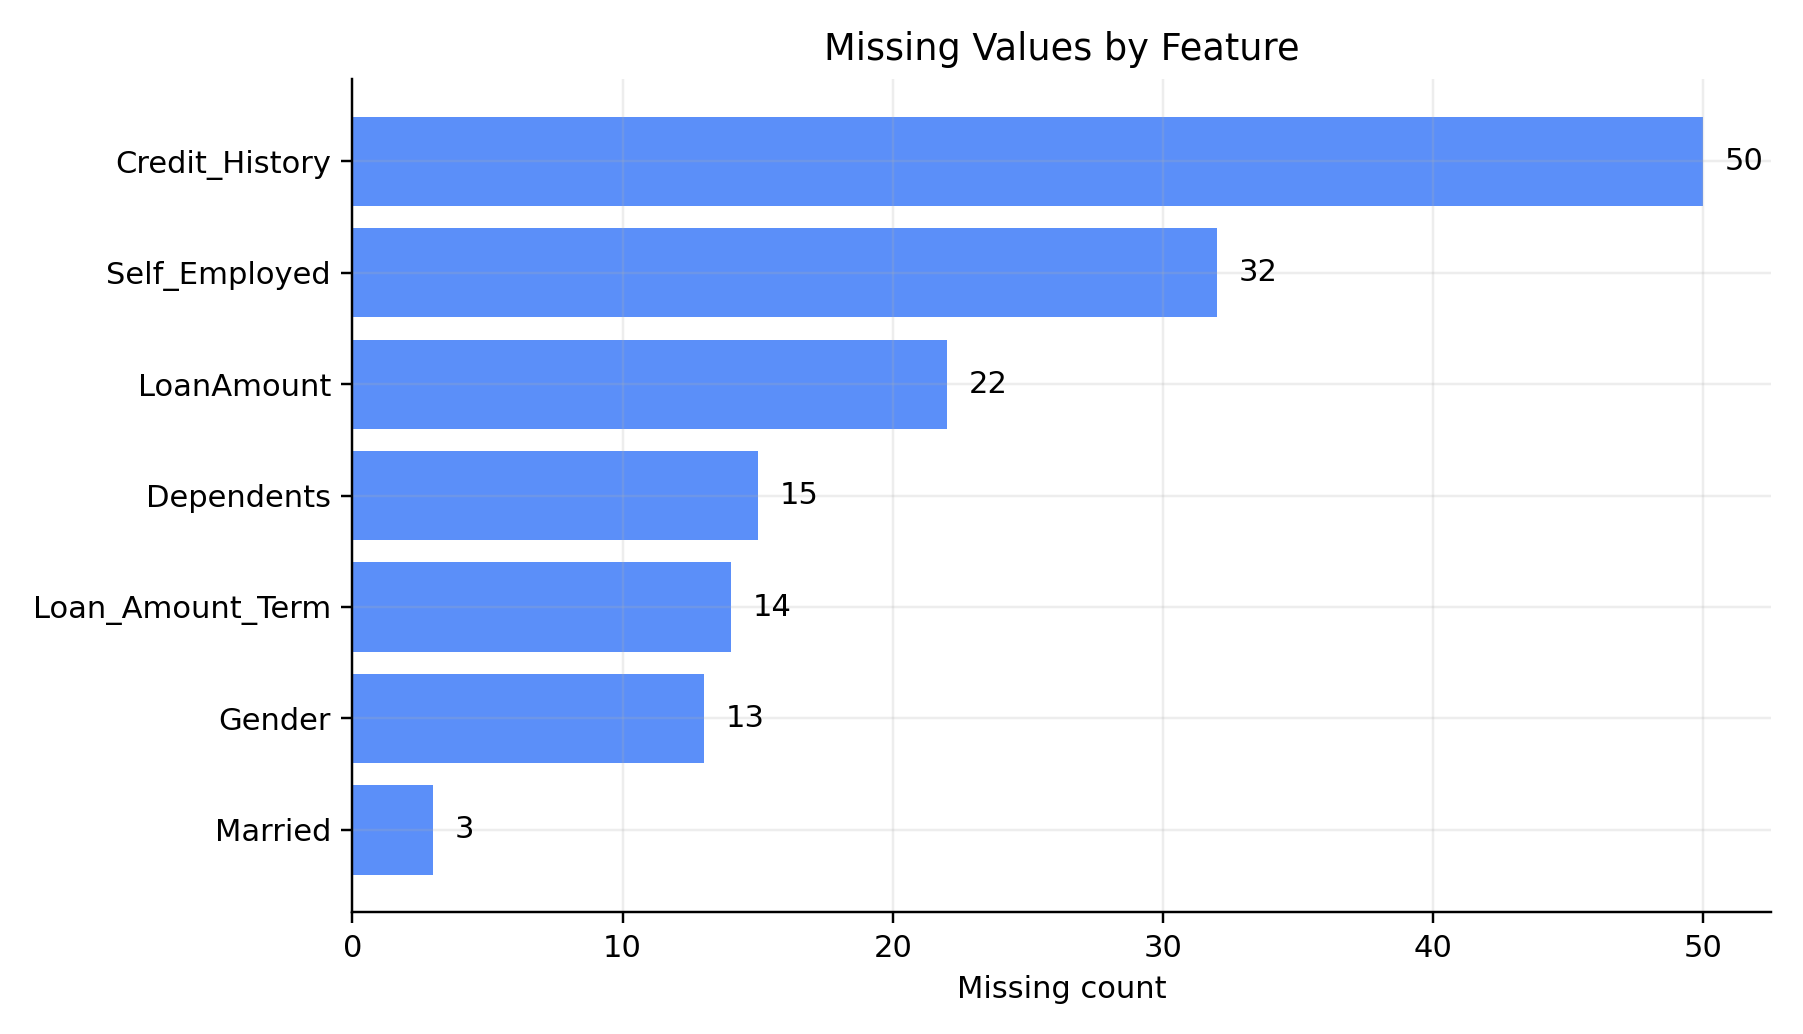
\includegraphics[width=0.82\linewidth]{figures/missing_values.png}
    \caption{各字段缺失值数量}
    \label{fig:missing}
\end{figure}

目标变量分布见图 \ref{fig:targetdist}。614 条记录中，贷款通过 \texttt{Y} 有 422 条，占 68.73\%；未通过 \texttt{N} 有 192 条，占 31.27\%。多数类基线在测试集上的准确率为 0.6911，但其宏平均 F1 仅为 0.4087，说明类别不均衡会显著影响仅看准确率时的判断。

\begin{figure}[H]
    \centering
    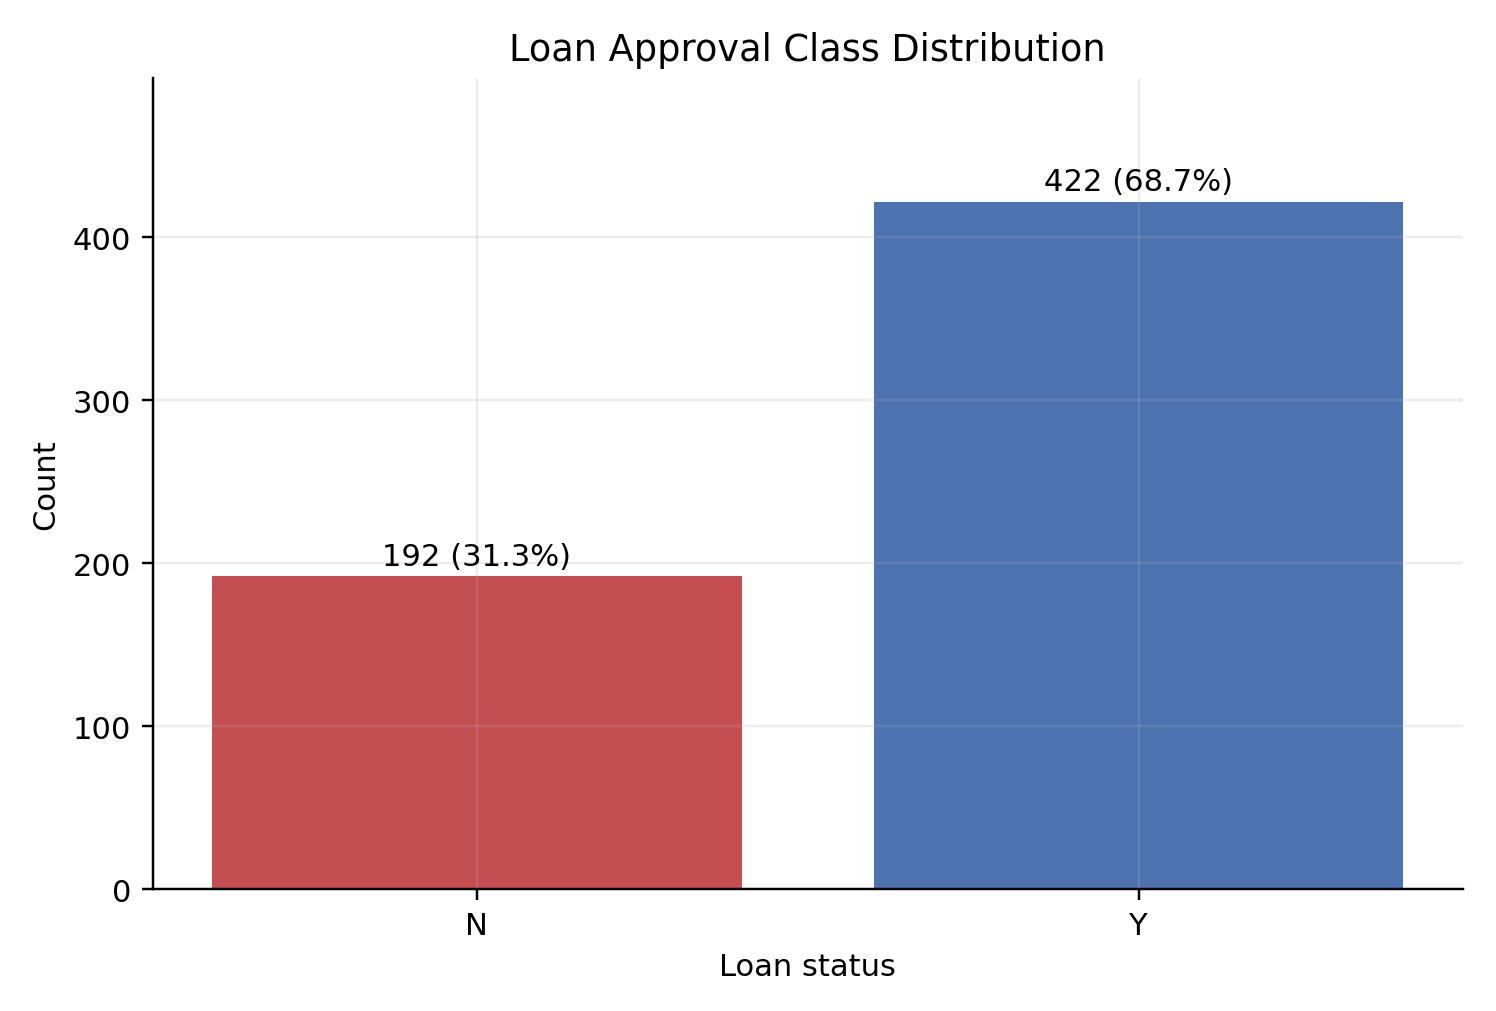
\includegraphics[width=0.66\linewidth]{figures/target_distribution.png}
    \caption{贷款审批结果类别分布}
    \label{fig:targetdist}
\end{figure}

\subsection{特征工程与算法实现}

原始收入和贷款金额具有明显右偏分布，而且贷款偿付能力通常取决于多个字段之间的比例关系。为此，本实验在原始变量基础上构造以下特征：

\begin{itemize}
    \item \texttt{Dependents\_Numeric}：将 \texttt{3+} 转换为 3，得到可计算的抚养人数。
    \item \texttt{TotalIncome}：申请人与共同申请人收入之和。
    \item \texttt{LogTotalIncome} 和 \texttt{LogLoanAmount}：对总收入和贷款金额进行对数变换，减弱极端值影响。
    \item \texttt{LoanIncomeRatio}：贷款金额与总收入的比值，用于近似刻画贷款负担。
    \item \texttt{InstallmentProxy}：贷款金额除以还款期限，作为每期偿还压力的近似量。
    \item \texttt{IncomePerDependent}：总收入除以家庭负担人数加一，近似反映人均可支配收入。
    \item \texttt{HasCoapplicant}：是否存在共同申请人收入。
    \item \texttt{CreditHistoryMissing}：信用历史是否缺失，保留缺失本身可能包含的信息。
\end{itemize}

数值特征采用中位数填补和标准化，类别特征采用众数填补和 One-Hot 编码。数据按照 80\%/20\% 分层随机划分为 491 条训练样本和 123 条测试样本，固定随机种子为 42。训练集内部使用 5 折分层交叉验证。模型和主要参数见表 \ref{tab:models}。

\begin{table}[H]
\centering
\caption{实验模型及主要参数}
\label{tab:models}
\small
\begin{tabular}{lll}
\toprule
模型 & 集成方式 & 主要设置\\
\midrule
\texttt{DecisionTree} & 单模型对照 & 最大深度 5，叶节点至少 8 条\\
\texttt{Bagging} & 并行集成 & 300 棵树，样本比例 0.85\\
\texttt{RandomForest} & 并行集成 & 500 棵树，平衡子采样类别权重\\
\texttt{ExtraTrees} & 强随机并行集成 & 500 棵树，叶节点至少 2 条\\
\texttt{AdaBoost} & 串行提升 & 220 个浅树，学习率 0.035\\
\texttt{GradientBoosting} & 梯度提升 & 250 棵浅树，学习率 0.03\\
\texttt{SoftVoting} & 异构概率融合 & 逻辑回归、随机森林、梯度提升\\
\bottomrule
\end{tabular}
\end{table}

程序实现流程如下：
\begin{enumerate}
    \item 读取 \texttt{loan.csv}，检查数据规模、字段类型、重复记录、缺失值和目标分布。
    \item 删除唯一编号 \texttt{Loan\_ID}，构造收入、贷款负担和缺失指示特征。
    \item 对数据进行 80\%/20\% 分层训练测试划分。
    \item 使用 \texttt{ColumnTransformer} 分别处理数值变量和类别变量，并将预处理与分类器封装为 \texttt{Pipeline}。
    \item 在训练集上进行 5 折分层交叉验证，计算 Accuracy、Macro-F1、Balanced Accuracy 和 ROC-AUC。
    \item 在固定测试集上比较各模型，绘制模型对比图和 ROC 曲线。
    \item 按训练集交叉验证 Macro-F1 选择最终模型，输出混淆矩阵、分类报告和置换重要性。
\end{enumerate}

完整 Python 程序见附录。

\section{实验结果与可扩展内容}

\subsection{探索性分析结果}

图 \ref{fig:numeric} 展示了主要数值变量在贷款通过和未通过两组中的分布。两组申请人收入均存在较大离散程度，仅依靠收入绝对值难以形成清晰边界。未通过组平均贷款金额为 151.22，通过组为 144.29，差异存在但并不十分显著；这说明贷款结果更可能取决于贷款金额与收入、信用历史等变量的组合，而不是某个单独数值。

\begin{figure}[H]
    \centering
    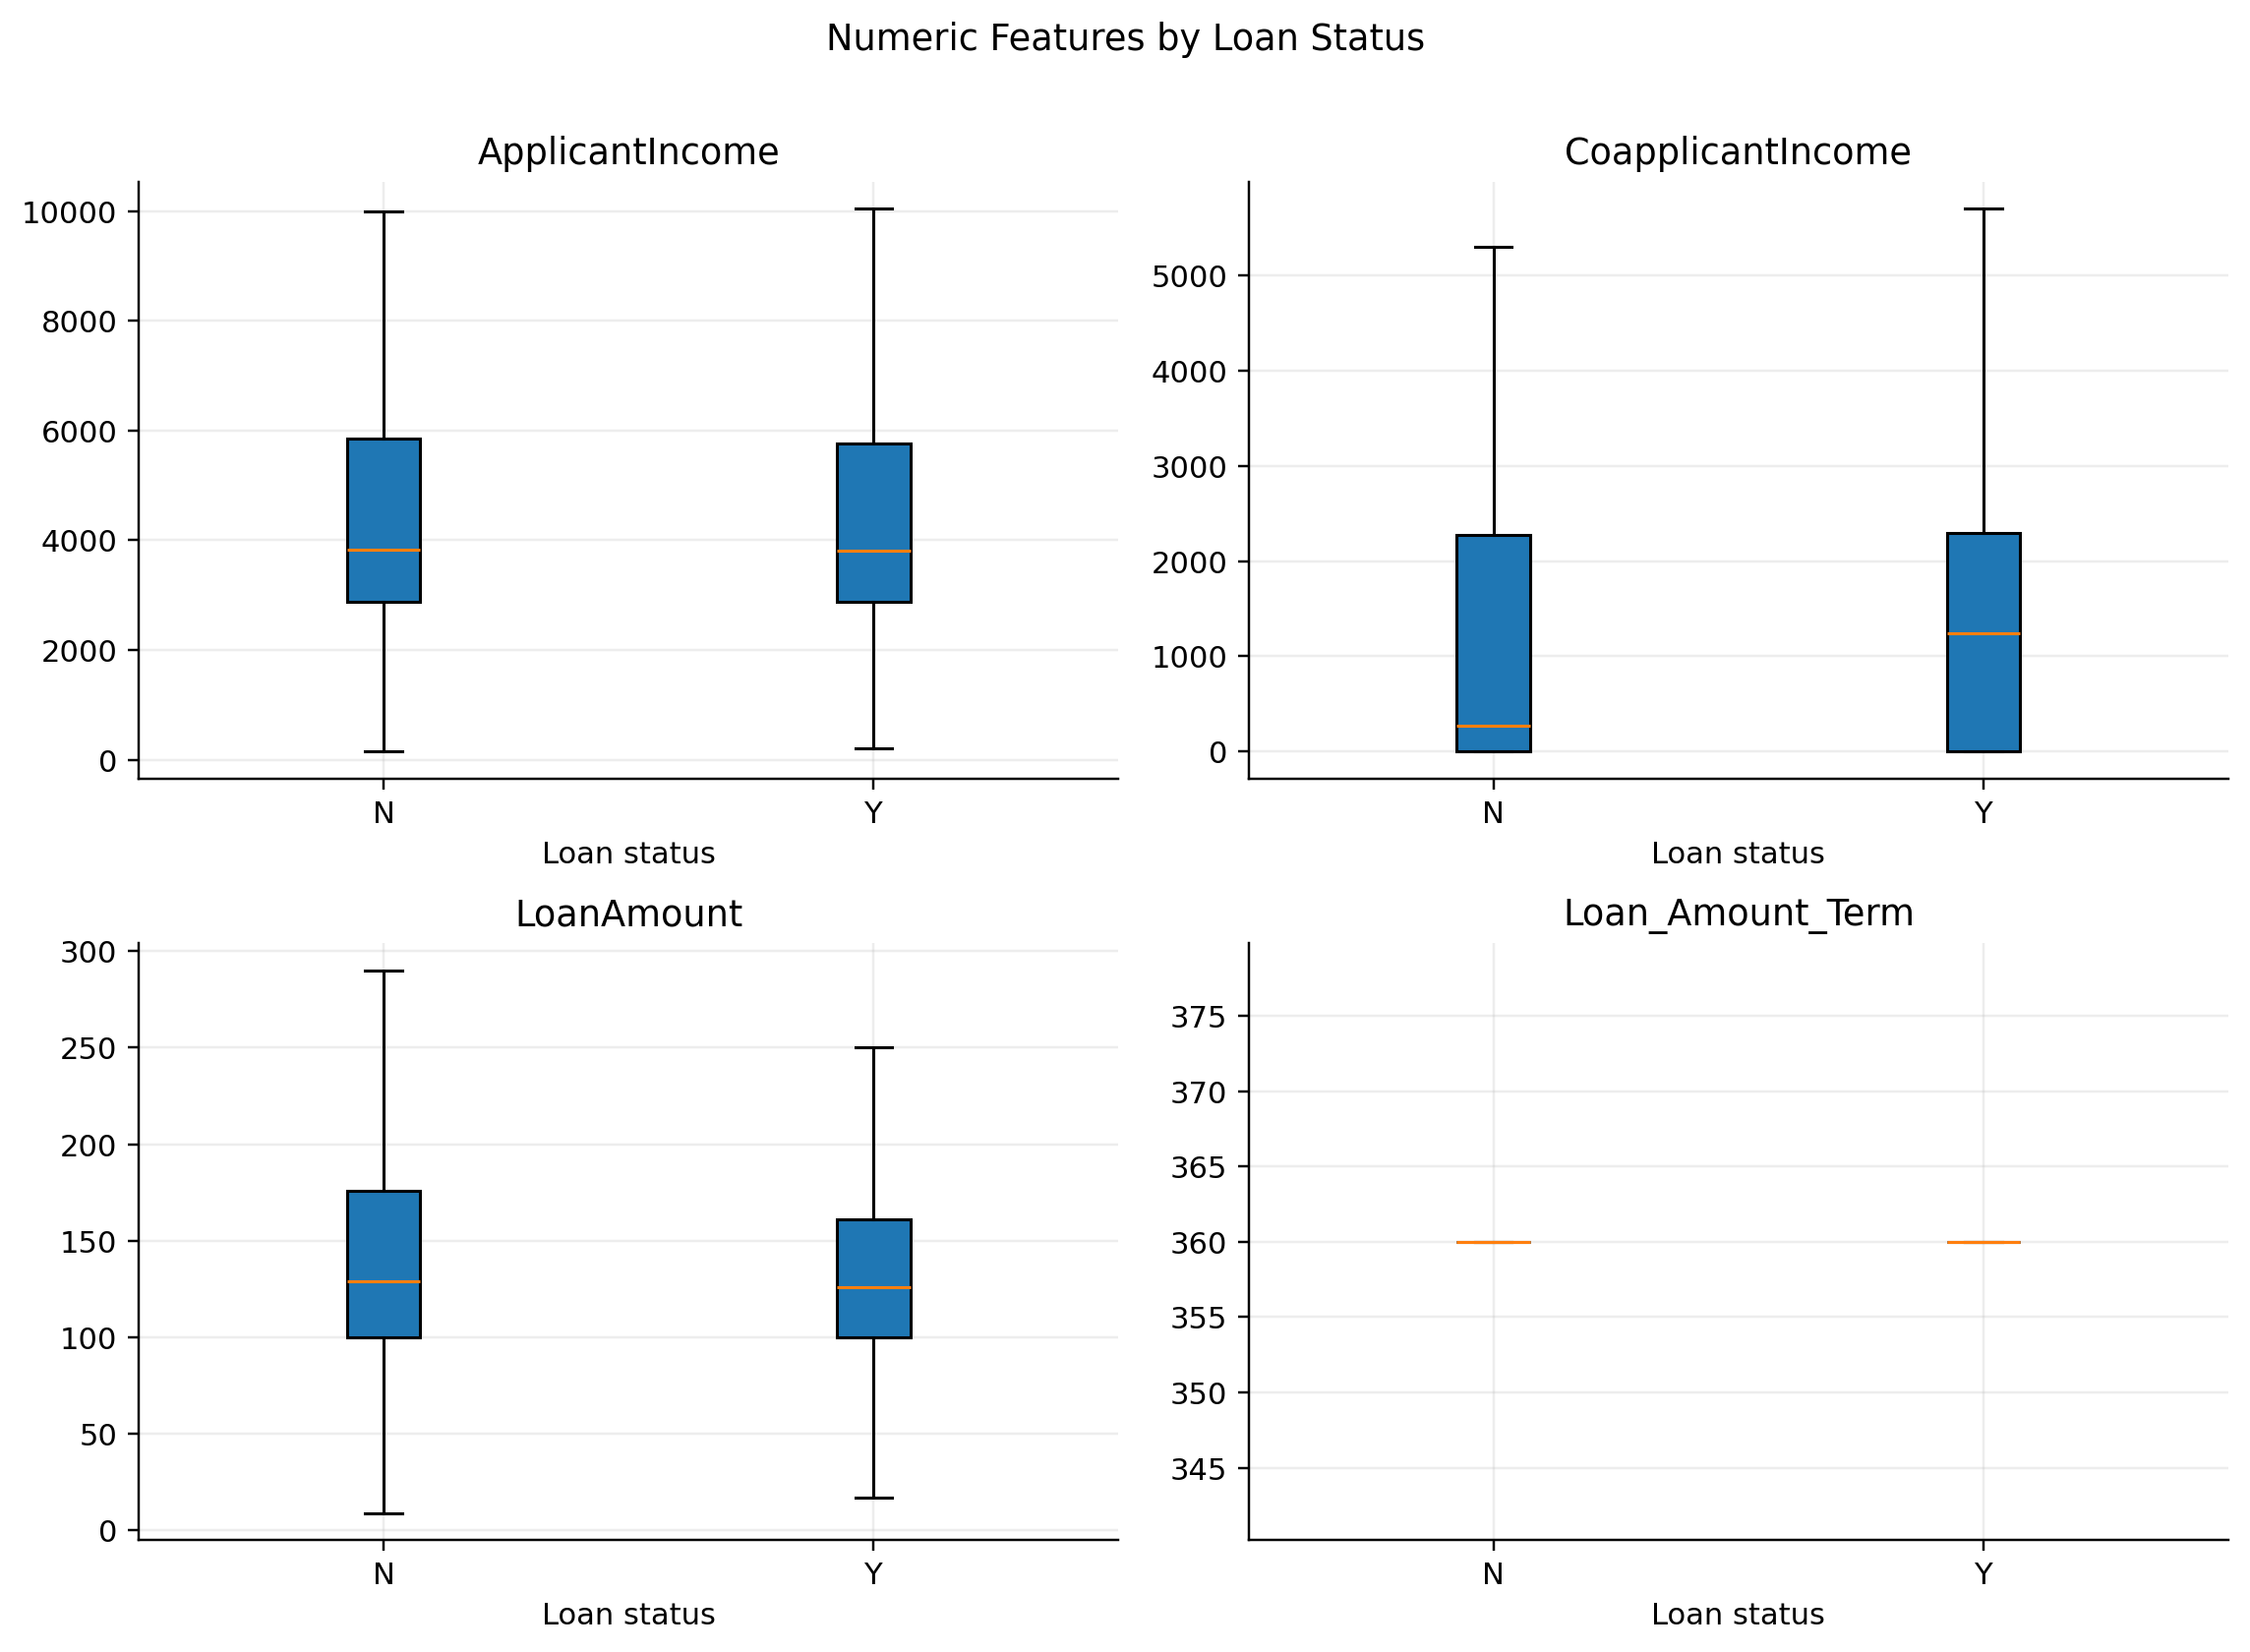
\includegraphics[width=0.92\linewidth]{figures/numeric_features_by_status.png}
    \caption{主要数值特征在不同贷款结果下的分布}
    \label{fig:numeric}
\end{figure}

选定类别特征与审批通过率的关系见图 \ref{fig:categoryrate}。\texttt{Credit\_History=1} 的申请人通过率为 79.58\%，而 \texttt{Credit\_History=0} 的申请人通过率仅为 7.87\%，差距非常明显。毕业生通过率为 70.83\%，非毕业生为 61.19\%；半城市房产申请人通过率为 76.82\%，高于城市的 65.84\% 和农村的 61.45\%。这些统计结果表明，信用历史是最重要的单一信号，教育和房产区域提供次要补充信息。

\begin{figure}[H]
    \centering
    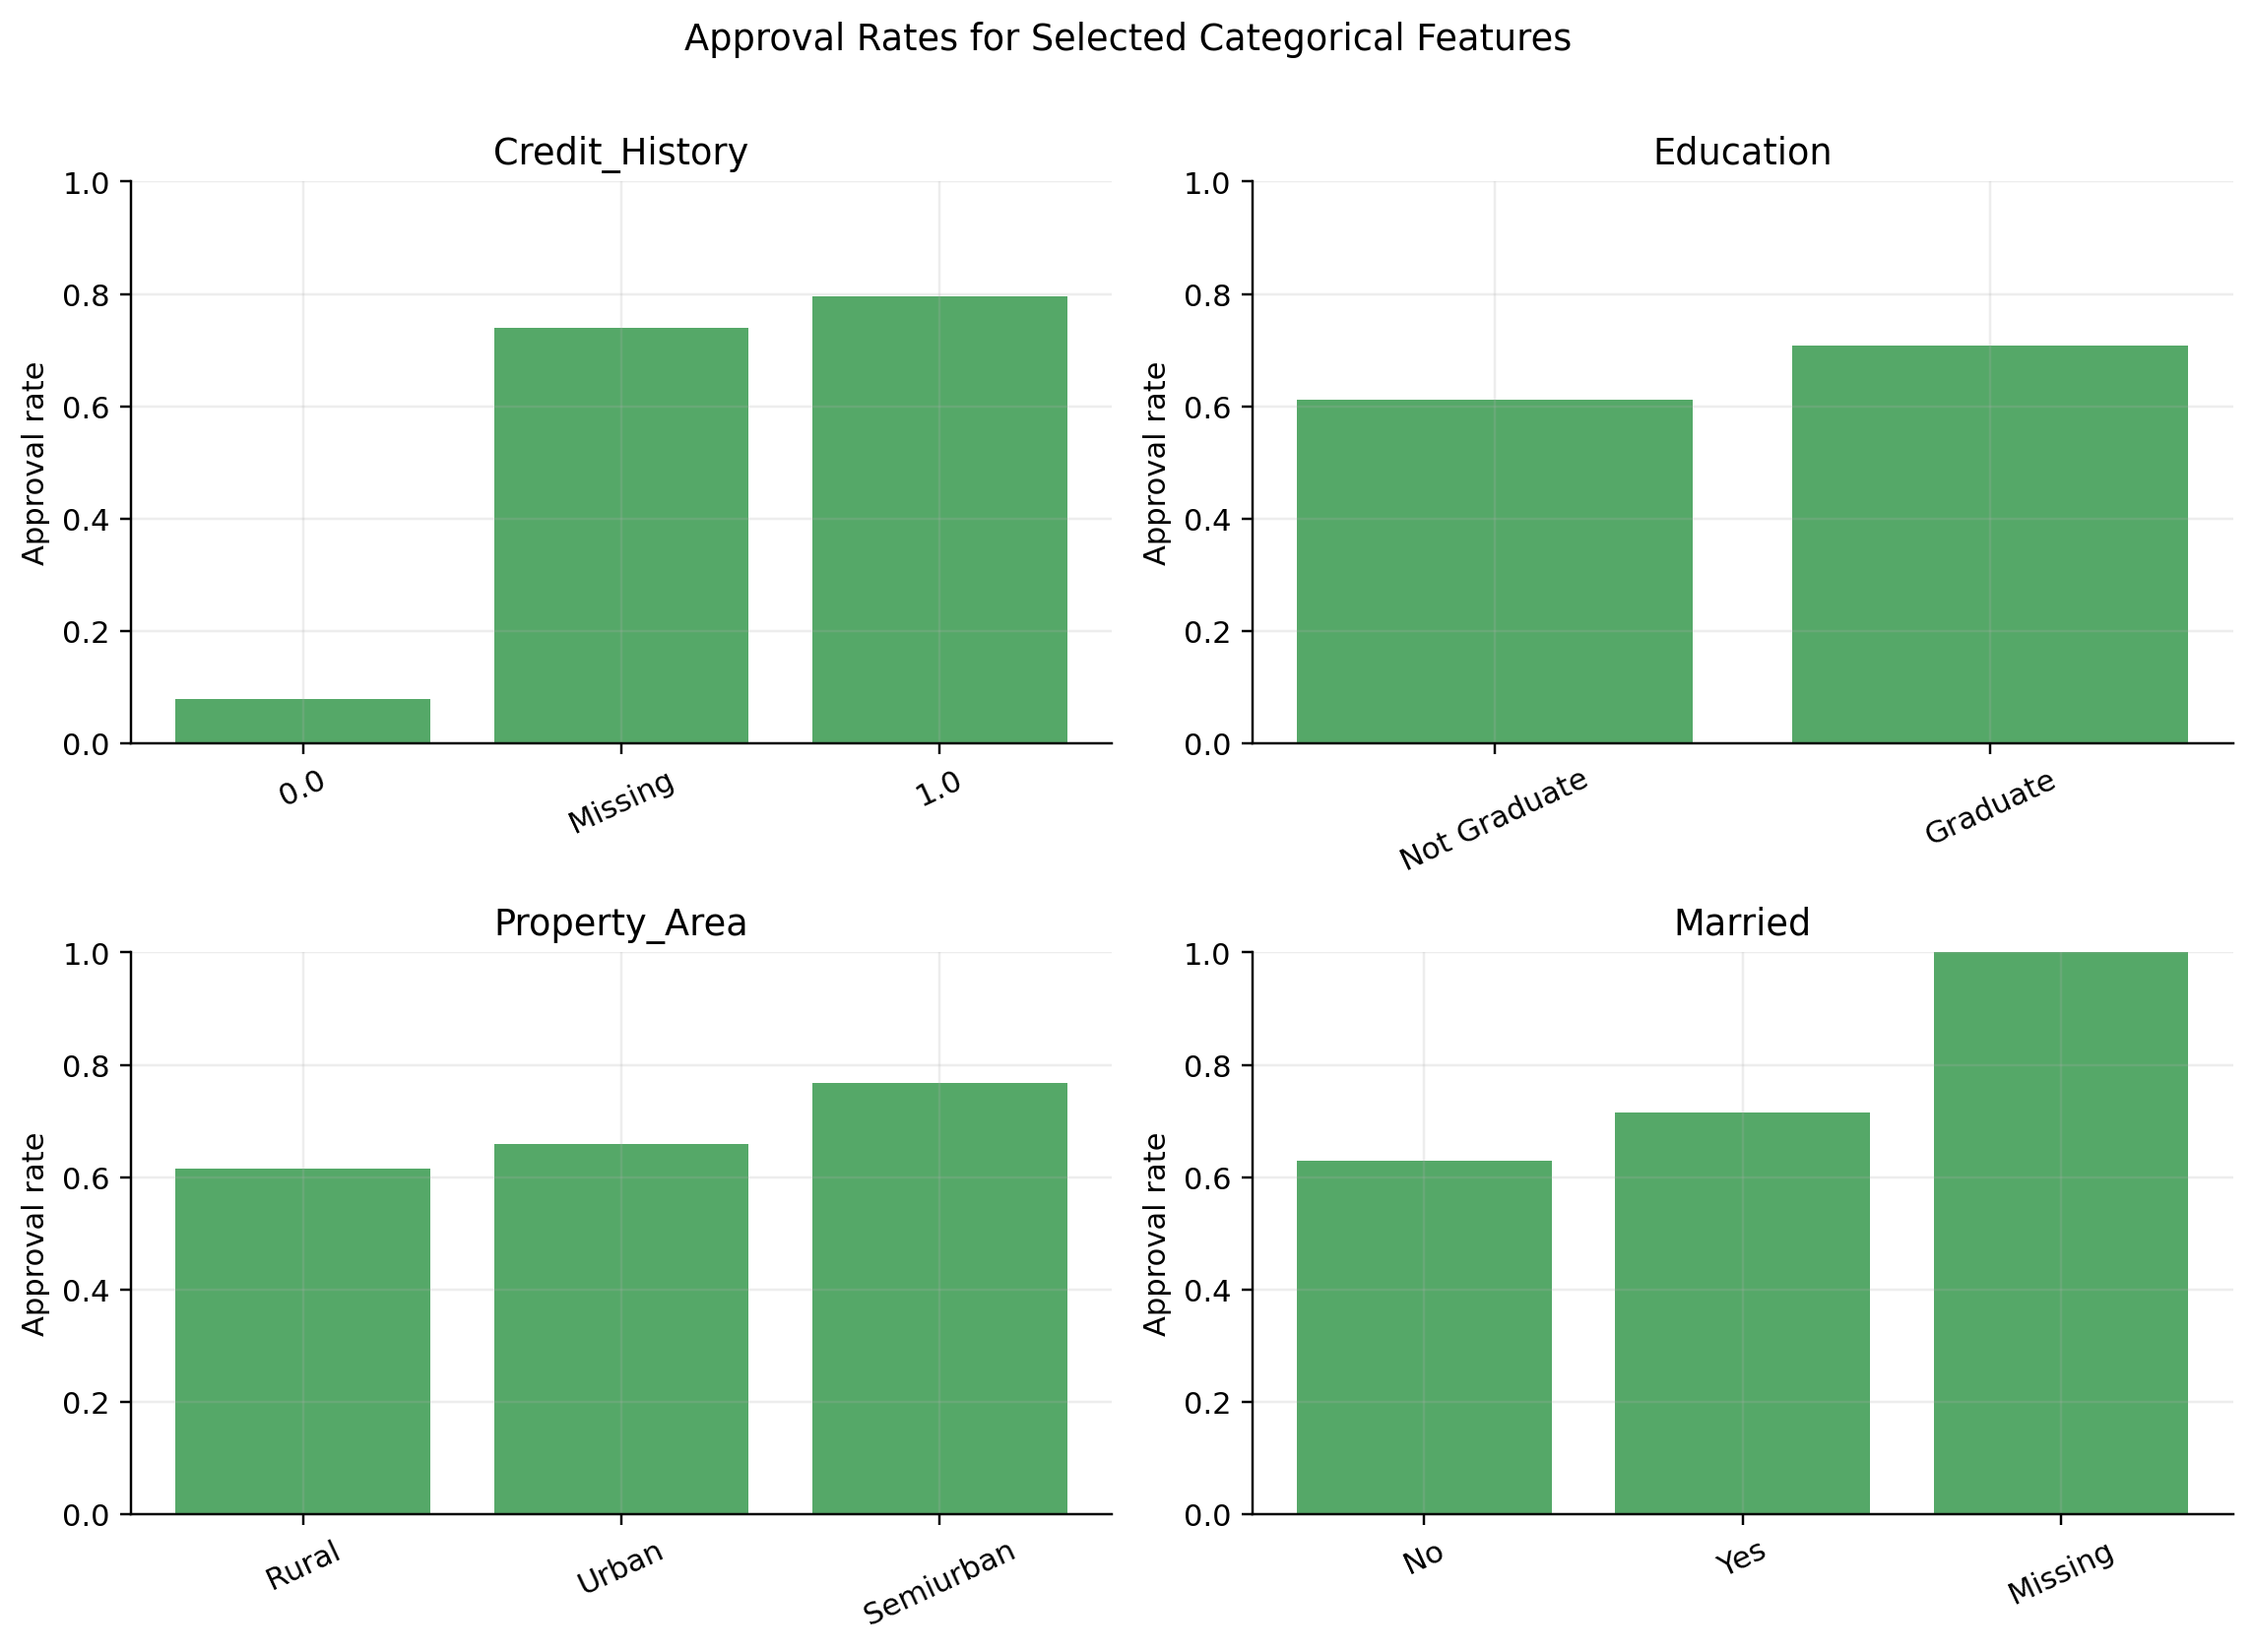
\includegraphics[width=0.93\linewidth]{figures/categorical_approval_rates.png}
    \caption{部分类别特征对应的贷款通过率}
    \label{fig:categoryrate}
\end{figure}

数值特征相关性热力图见图 \ref{fig:corr}。\texttt{ApplicantIncome} 与 \texttt{TotalIncome} 高度相关，\texttt{LoanAmount} 与对数贷款金额也高度相关，这是特征工程的预期结果。树模型可以从不同尺度和非线性切分中自动选择有效表达，因此保留这些变量用于比较；置换重要性则在最终解释时衡量每个原始或构造特征对泛化性能的实际贡献。

\begin{figure}[H]
    \centering
    
\includegraphics[width=0.9\linewidth]{figures/correlation_heatmap.png}
    \caption{数值变量及构造特征相关性热力图}
    \label{fig:corr}
\end{figure}

\subsection{模型比较结果}

各模型测试集结果见表 \ref{tab:testresult}。软投票模型在本次固定测试集上表现最好，Accuracy 为 0.9024，Macro-F1 为 0.8802，ROC-AUC 为 0.8833。梯度提升测试集 Accuracy 为 0.8780，Macro-F1 为 0.8489。Bagging、随机森林和 AdaBoost 也明显优于多数类基线。单棵决策树 Macro-F1 为 0.8011，而多个集成模型达到 0.81 以上，说明组合多个基学习器能够改善总体分类性能。

\begin{table}[H]
\centering
\caption{各模型测试集评价结果}
\label{tab:testresult}
\small
\begin{tabular}{lrrrr}
\toprule
模型 & Accuracy & Bal. Acc. & Macro-F1 & ROC-AUC\\
\midrule
\texttt{SoftVoting} & 0.9024 & 0.8639 & 0.8802 & 0.8833\\
\texttt{GradientBoosting} & 0.8780 & 0.8317 & 0.8489 & 0.8808\\
\texttt{Bagging} & 0.8699 & 0.8477 & 0.8477 & 0.8669\\
\texttt{RandomForest} & 0.8537 & 0.8286 & 0.8286 & 0.8582\\
\texttt{AdaBoost} & 0.8374 & 0.8096 & 0.8096 & 0.9203\\
\texttt{DecisionTree} & 0.8211 & 0.8197 & 0.8011 & 0.8839\\
\texttt{ExtraTrees} & 0.7967 & 0.7511 & 0.7565 & 0.8121\\
\texttt{Majority\_Baseline} & 0.6911 & 0.5000 & 0.4087 & 0.5000\\
\bottomrule
\end{tabular}
\end{table}

图 \ref{fig:modelcompare} 同时给出测试集和交叉验证 Macro-F1。可以看到，软投票在测试集上的分数明显高于其交叉验证均值，说明本次测试划分可能较有利于该模型。如果仅根据测试集最高分选择模型，就会对一次随机划分产生过度依赖。因此，本实验预先规定按训练集 5 折交叉验证 Macro-F1 选择最终模型，测试集仅用于最终估计。

\begin{figure}[H]
    \centering
    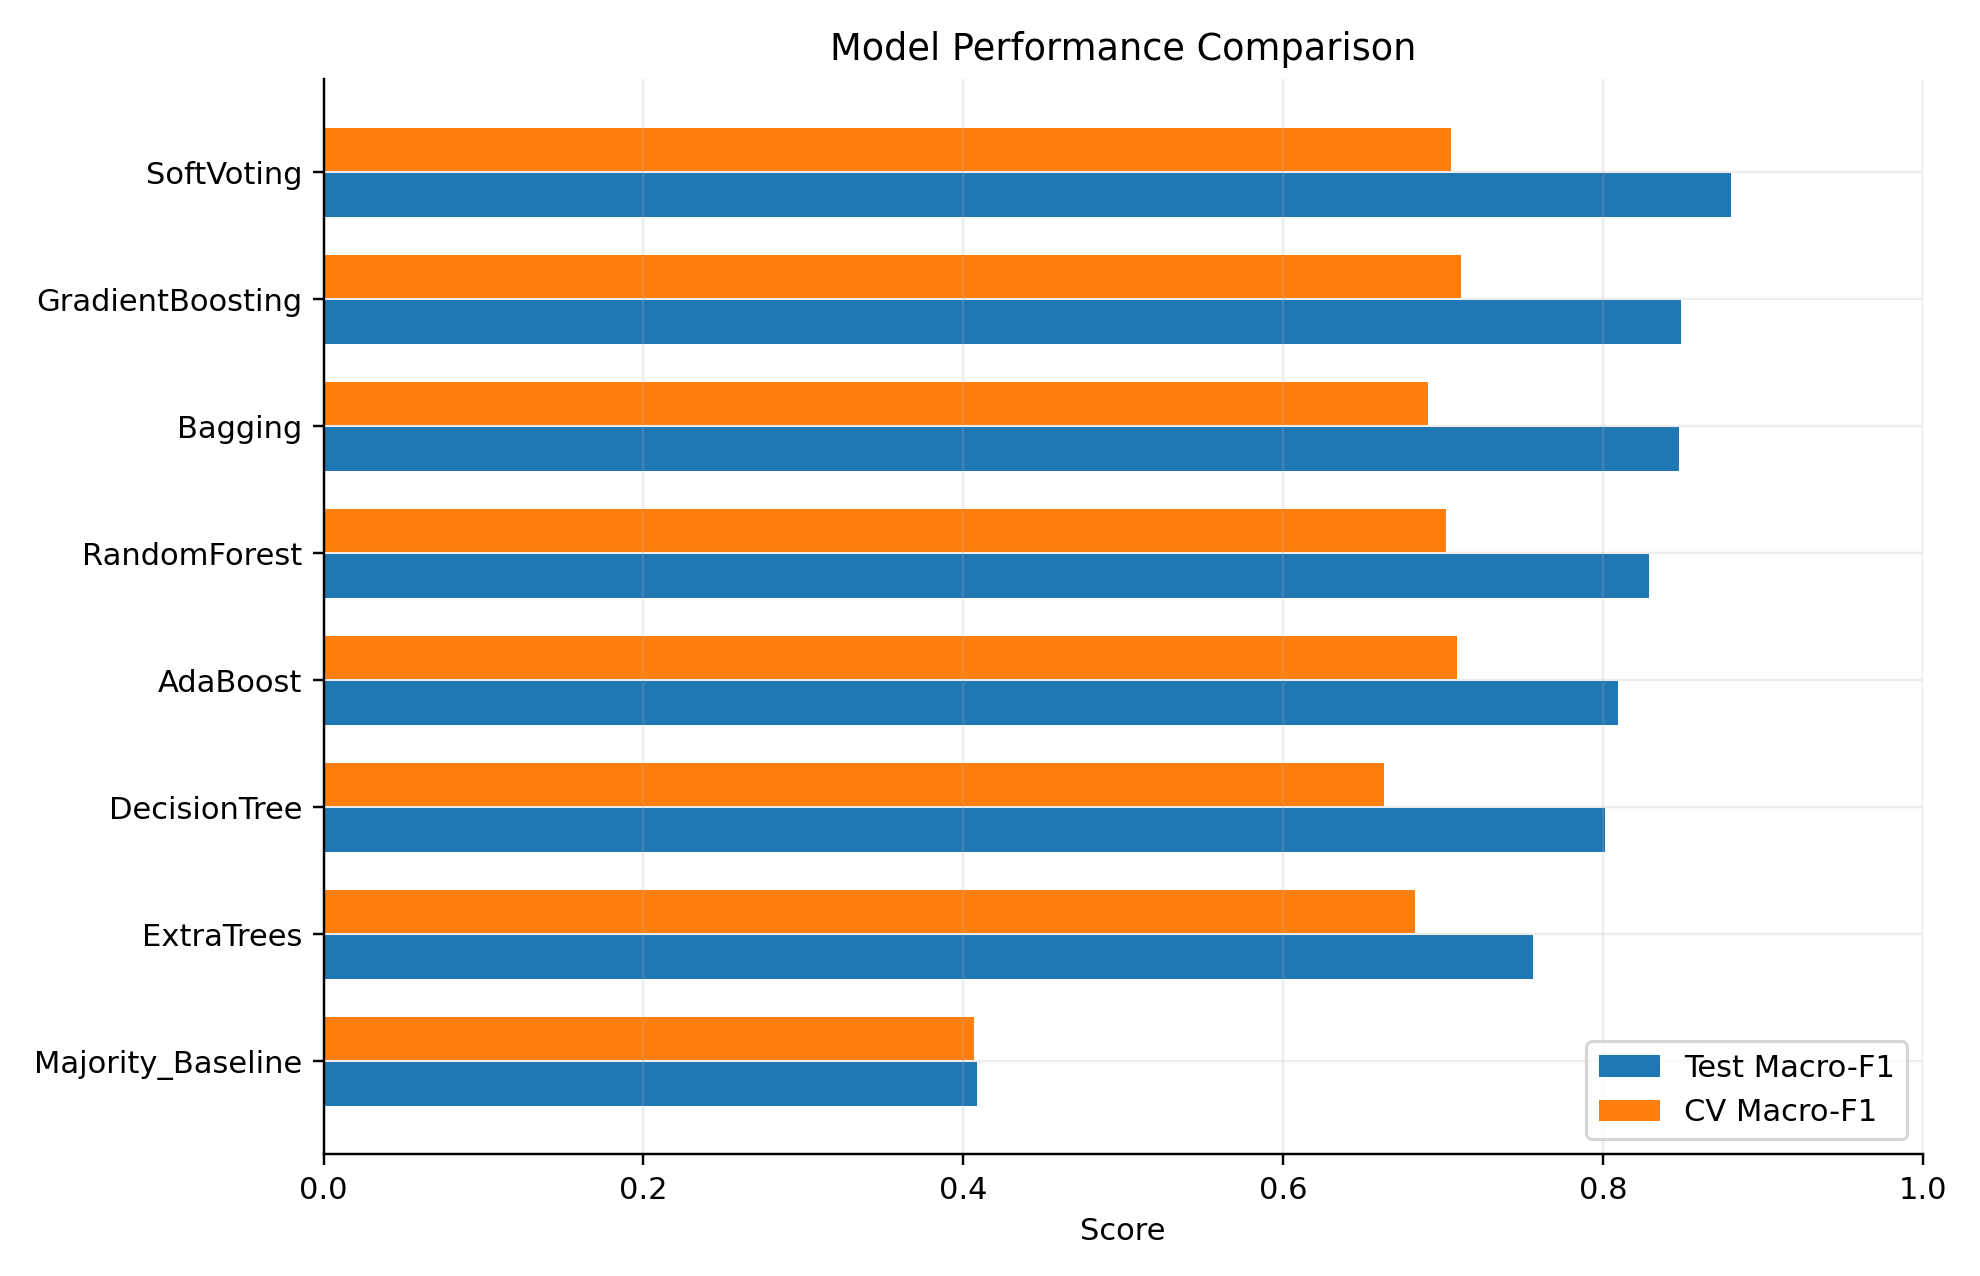
\includegraphics[width=0.9\linewidth]{figures/model_comparison.png}
    \caption{各模型测试集与交叉验证 Macro-F1 对比}
    \label{fig:modelcompare}
\end{figure}

5 折交叉验证结果见表 \ref{tab:cvresult}。梯度提升平均 Macro-F1 为 0.7115，略高于 AdaBoost 的 0.7088、软投票的 0.7049 和随机森林的 0.7021，因此被选为最终模型。前四个模型均值差距很小，而标准差约为 0.09--0.10，说明数据规模较小，不同折之间仍存在明显波动。较谨慎的结论应是：Boosting、软投票和随机森林都属于较可靠的候选方案，而不是某个模型具有压倒性优势。

\begin{table}[H]
\centering
\caption{模型 5 折分层交叉验证结果}
\label{tab:cvresult}
\small
\begin{tabular}{lrrrr}
\toprule
模型 & CV Accuracy & CV Bal. Acc. & CV Macro-F1 & CV ROC-AUC\\
\midrule
\texttt{GradientBoosting} & 0.7921 & 0.6954 & 0.7115 & 0.7740\\
\texttt{AdaBoost} & 0.7860 & 0.6948 & 0.7088 & 0.7321\\
\texttt{SoftVoting} & 0.7840 & 0.6913 & 0.7049 & 0.7784\\
\texttt{RandomForest} & 0.7759 & 0.6925 & 0.7021 & 0.7716\\
\texttt{Bagging} & 0.7657 & 0.6816 & 0.6907 & 0.7748\\
\texttt{ExtraTrees} & 0.7413 & 0.6779 & 0.6827 & 0.7156\\
\texttt{DecisionTree} & 0.7109 & 0.6642 & 0.6630 & 0.6994\\
\texttt{Majority\_Baseline} & 0.6864 & 0.5000 & 0.4070 & 0.5000\\
\bottomrule
\end{tabular}
\end{table}

测试集 ROC 曲线见图 \ref{fig:roc}。所有有效模型的 ROC-AUC 均明显高于随机分类器。AdaBoost 的测试集 ROC-AUC 最高，为 0.9203，但其默认 0.5 阈值下的 Macro-F1 为 0.8096。这说明“概率排序能力”和“固定阈值分类效果”并不完全相同。实际金融应用中可以根据误批和拒批成本重新调整阈值，而本报告为了公平比较，所有模型均使用默认分类规则。

\begin{figure}[H]
    \centering
    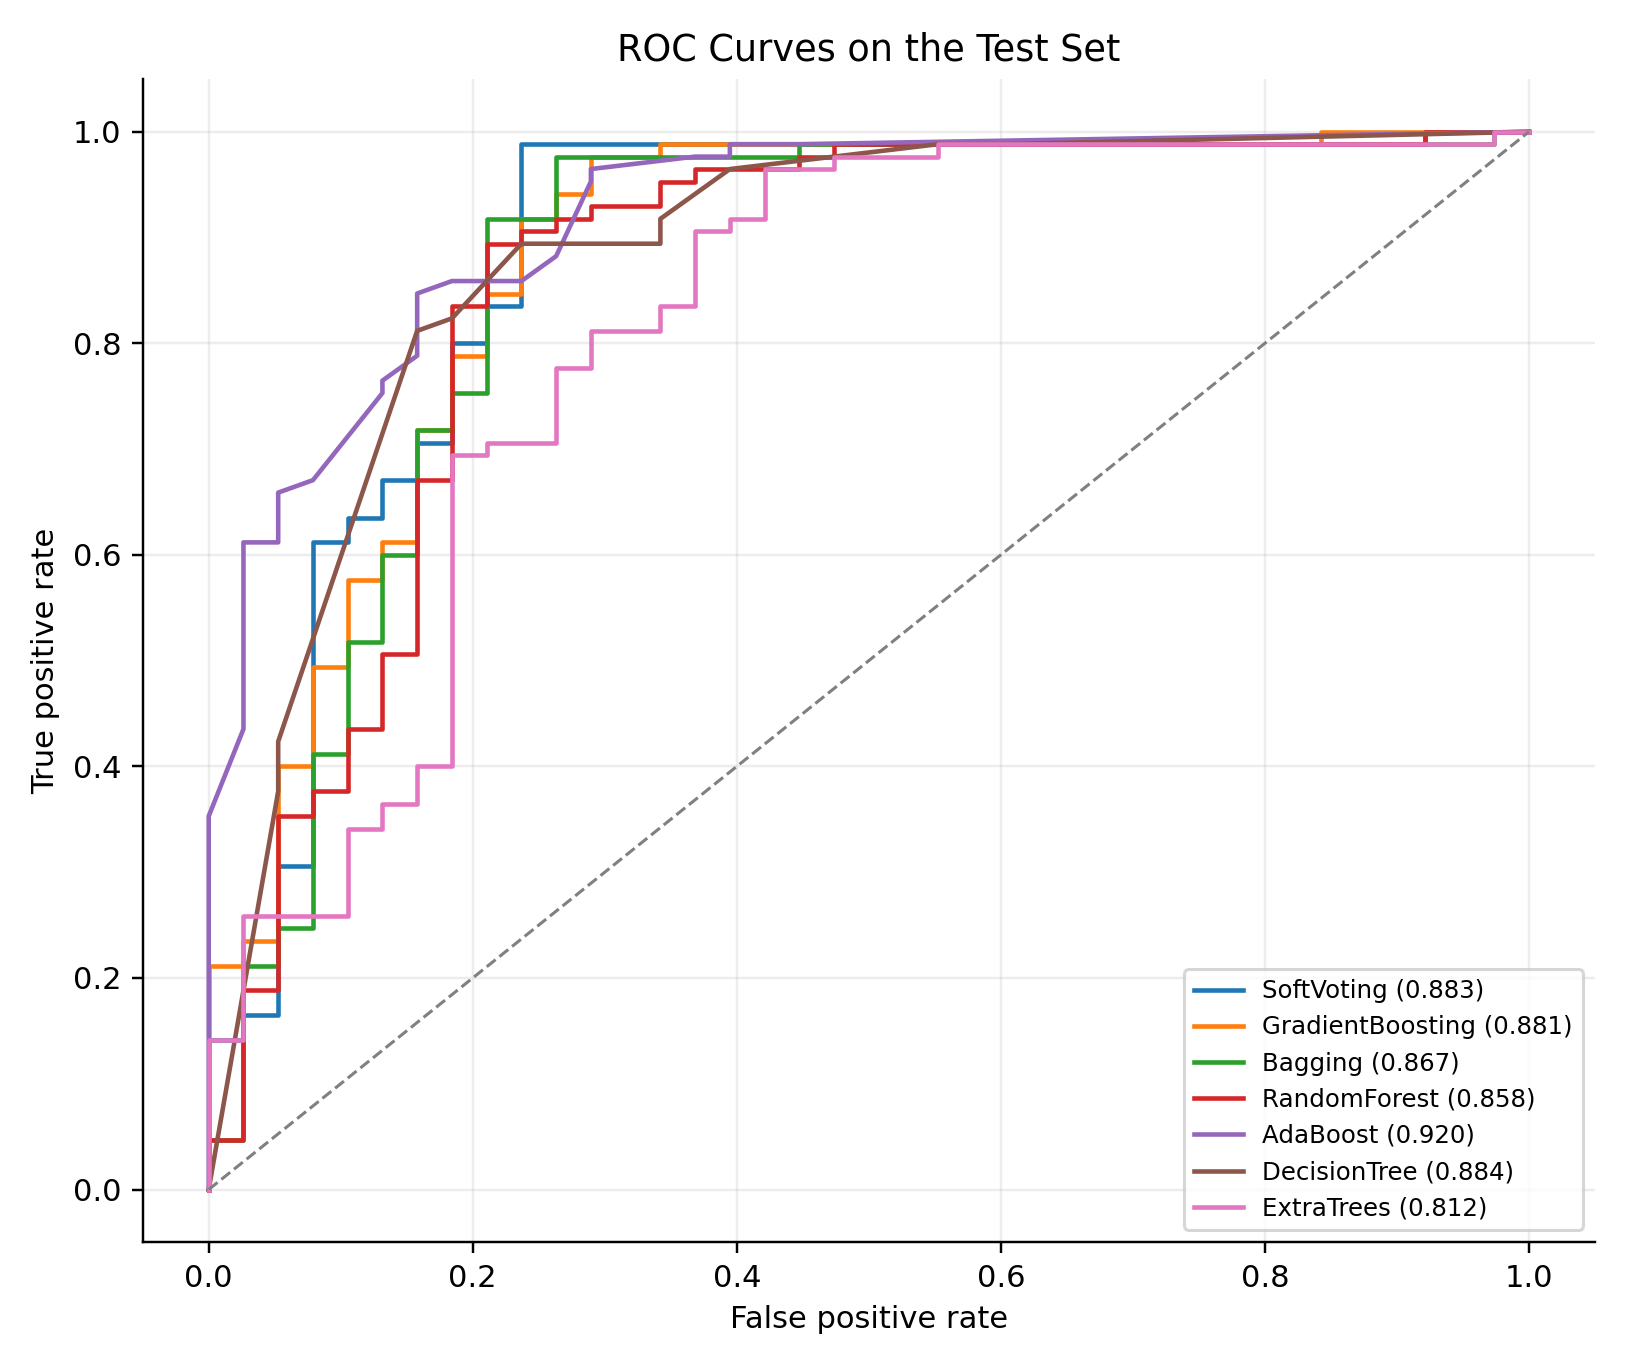
\includegraphics[width=0.78\linewidth]{figures/roc_curves.png}
    \caption{各集成模型测试集 ROC 曲线}
    \label{fig:roc}
\end{figure}

\subsection{最终模型分析}

按交叉验证选择的梯度提升模型在测试集上正确分类 108 条、错误分类 15 条，混淆矩阵见图 \ref{fig:cm}。38 条实际未通过申请中，模型正确识别 27 条，误批 11 条；85 条实际通过申请中，模型正确识别 81 条，误拒 4 条。未通过类的 Precision 为 0.8710、Recall 为 0.7105、F1 为 0.7826；通过类的 Precision 为 0.8804、Recall 为 0.9529、F1 为 0.9153。

\begin{figure}[H]
    \centering
    
\includegraphics[width=0.61\linewidth]{figures/best_confusion_matrix.png}
    \caption{梯度提升模型测试集混淆矩阵}
    \label{fig:cm}
\end{figure}

模型对通过类的召回率较高，能够识别绝大多数历史上获得贷款的申请，但未通过类召回率相对较低。在实际风险控制场景中，误将高风险申请预测为通过通常比误拒低风险申请造成更大损失，因此可以适当提高通过阈值，或使用代价敏感学习对误批赋予更高惩罚。当前实验主要用于验证集成学习方法，不对业务成本进行主观设定。

置换重要性见图 \ref{fig:importance}。\texttt{Credit\_History} 的重要性远高于其他变量，随机打乱后测试集 Macro-F1 平均下降约 0.2652；\texttt{LoanIncomeRatio} 排名第二，下降约 0.0724；\texttt{Property\_Area} 排名第三。该结果与探索性分析一致：历史信用是否合规是贷款审批的核心信号，而贷款金额相对于家庭总收入的负担比单独收入或单独贷款金额更有解释力。

\begin{figure}[H]
    \centering
    
\includegraphics[width=0.9\linewidth]{figures/feature_importance_top20.png}
    \caption{梯度提升模型置换重要性}
    \label{fig:importance}
\end{figure}

需要说明的是，置换重要性表示特征对当前模型预测性能的贡献，不等同于因果关系。例如，信用历史可能与其他未记录的经济条件相关，不能据此断言改变某个字段一定会直接改变审批结果。此外，性别、婚姻和教育等字段涉及公平性问题，即使在当前数据中贡献有限，真实部署前也应进行分组准确率、机会均等和差别影响审计。

\subsection{参数调优及可扩展内容}

本次实验采用一组合理固定参数完成模型对比，避免在较小数据集上进行过度搜索。后续可从以下方向扩展：

\begin{itemize}
    \item 使用嵌套交叉验证调节梯度提升的树深、学习率、弱学习器数量和最小叶节点样本数，得到偏差更小的泛化估计。
    \item 使用重复分层交叉验证，降低单次 5 折划分造成的方差，并报告置信区间。
    \item 根据银行的误批与误拒成本设计代价矩阵，通过阈值搜索或类别权重优化业务目标，而不局限于默认 0.5 阈值。
    \item 尝试 XGBoost、LightGBM 或 CatBoost 等更成熟的提升算法，并使用早停控制过拟合。
    \item 对概率输出进行 Platt scaling 或等距回归校准，使预测概率更接近真实违约或审批频率。
    \item 按性别、婚姻、教育和房产区域分别计算召回率与误报率，检查模型是否对特定群体产生系统性不利影响。
    \item 收集负债、职业稳定性、资产、历史还款行为等更直接的偿付能力变量，提高预测效果和业务解释性。
\end{itemize}

\section{讨论与结论}

\subsection{结果讨论}

第一，集成学习整体优于简单基线。多数类模型的 Accuracy 看似达到 0.6911，但无法识别未通过类，Macro-F1 只有 0.4087。单棵决策树将测试集 Macro-F1 提高到 0.8011，而软投票、梯度提升、Bagging 和随机森林进一步达到 0.8286--0.8802，说明多学习器组合能够有效利用贷款申请特征。

第二，不同集成方式各有特点。Bagging 和随机森林通过平均多棵树降低方差，表现稳定；梯度提升和 AdaBoost 逐步修正错误样本，在交叉验证中位居前列；软投票能够融合线性和非线性模型，在固定测试集上取得最高分。但软投票测试分数与交叉验证均值之间存在较大差距，因此不能只看单次测试结果。

第三，信用历史是最关键的预测特征。具有合规信用历史的申请人通过率接近 80\%，没有合规信用历史的申请人通过率不足 8\%。置换重要性同样显示 \texttt{Credit\_History} 对 Macro-F1 的影响远高于其他字段。贷款收入比位居第二，表明相对负担比收入或贷款金额的绝对值更能反映审批风险。

第四，模型仍然存在类别不对称。最终梯度提升模型对通过类的召回率为 0.9529，对未通过类的召回率为 0.7105。由于误批可能带来信用损失，实际应用应针对业务成本选择阈值，并由人工复核边界样本，而不能直接把模型输出作为最终审批决定。

\subsection{结论总结}

本次实验完成了基于贷款申请数据的集成分类任务。实验从数据读取开始，依次完成缺失值检查、探索性分析、特征工程、预处理管线构建、训练测试划分、5 折交叉验证、模型比较和结果解释。通过比较决策树、Bagging、随机森林、极端随机树、AdaBoost、梯度提升和软投票模型，验证了集成学习相对于多数类基线和单棵决策树的优势。

软投票模型在固定测试集上取得最高结果，Accuracy 为 0.9024，Macro-F1 为 0.8802；按训练集交叉验证 Macro-F1 选择的最终模型为梯度提升，其测试集 Accuracy 为 0.8780，Macro-F1 为 0.8489，ROC-AUC 为 0.8808。最终模型正确识别 27 条未通过申请和 81 条通过申请。综合分析表明，信用历史、贷款收入比和房产区域是当前数据中最有价值的预测信息。

总体而言，集成模型可以为贷款审批提供有效辅助，但 614 条样本仍不足以支持直接部署。模型结果应与业务规则、人工审核、公平性评估和概率校准结合使用。特别是涉及性别、婚姻和教育等敏感或代理变量时，需要确保模型不会把历史审批偏差固化为自动化决策。

\section{心得体会与思考}

\subsection{个人心得}

通过本次实验，我对 Bagging、随机森林、Boosting 和投票集成之间的差异有了更直观的理解。它们都叫作集成学习，但解决问题的方式不同：Bagging 更强调通过并行抽样降低方差，Boosting 更强调连续修正前一轮错误，投票集成则利用不同模型的互补性。只有同时观察交叉验证、测试集和混淆矩阵，才能判断某个高分究竟来自稳定能力还是一次数据划分的偶然性。

本次实验也让我进一步认识到预处理管线的重要性。如果先在完整数据集上填补缺失值或标准化，再做交叉验证，验证折的信息就会间接进入训练过程。把预处理和模型统一放入 \texttt{Pipeline} 后，每个训练折都独立估计填补值和编码规则，实验结果更可信，也更容易复现。

\subsection{启发与思考}

贷款审批不是只追求准确率的普通分类问题。不同错误的成本并不相同，误批可能造成资金损失，误拒则可能损害客户体验并错失业务机会。因此，真实系统应该先明确成本和监管要求，再选择评价指标与决策阈值。测试集上 AdaBoost 的 ROC-AUC 很高但默认阈值 F1 并非最高，正好说明概率排序和最终决策需要分开考虑。

此外，模型可解释性不能只停留在“哪个变量最重要”。信用历史的重要性很高，但模型预测仍然是相关性结果。对于性别、婚姻和教育等变量，还必须考虑公平性和合法合规问题。机器学习适合帮助审核人员组织信息、提示风险和提高效率，但不应取代对个人情况的综合判断，也不应成为无法申诉的黑箱决定。

\clearpage
\section{附录}

\subsection*{算法代码及其注释}
\addcontentsline{toc}{subsection}{算法代码及其注释}

\VerbatimInput[breaklines,breakanywhere,fontsize=\small,frame=single,rulecolor=\color{gray!45}]{report_code.py}

\clearpage
\subsection*{关键运行结果汇总}
\addcontentsline{toc}{subsection}{关键运行结果汇总}

\begin{Verbatim}[breaklines,breakanywhere,fontsize=\footnotesize,frame=single,rulecolor=\color{gray!45}]
数据规模：(614, 13)
原始输入字段：11 个（删除 Loan_ID，Loan_Status 为目标）
缺失单元格：149
训练集样本数：491
测试集样本数：123

类别分布：
Y：422（68.73%）
N：192（31.27%）

测试集模型结果：
SoftVoting           Accuracy=0.9024, Macro-F1=0.8802, ROC-AUC=0.8833
GradientBoosting     Accuracy=0.8780, Macro-F1=0.8489, ROC-AUC=0.8808
Bagging              Accuracy=0.8699, Macro-F1=0.8477, ROC-AUC=0.8669
RandomForest         Accuracy=0.8537, Macro-F1=0.8286, ROC-AUC=0.8582
AdaBoost             Accuracy=0.8374, Macro-F1=0.8096, ROC-AUC=0.9203
DecisionTree         Accuracy=0.8211, Macro-F1=0.8011, ROC-AUC=0.8839
ExtraTrees           Accuracy=0.7967, Macro-F1=0.7565, ROC-AUC=0.8121
Majority_Baseline    Accuracy=0.6911, Macro-F1=0.4087, ROC-AUC=0.5000

训练集 5 折交叉验证 Macro-F1：
GradientBoosting=0.7115
AdaBoost=0.7088
SoftVoting=0.7049
RandomForest=0.7021
Bagging=0.6907
ExtraTrees=0.6827
DecisionTree=0.6630
Majority_Baseline=0.4070

最终模型：GradientBoosting（按交叉验证 Macro-F1 选择）
测试集分类报告：
N：precision=0.8710, recall=0.7105, f1-score=0.7826, support=38
Y：precision=0.8804, recall=0.9529, f1-score=0.9153, support=85

混淆矩阵：
       预测N  预测Y
真实N    27     11
真实Y     4     81

置换重要性前三：
Credit_History=0.2652
LoanIncomeRatio=0.0724
Property_Area=0.0102
\end{Verbatim}

\end{document}
